\documentclass{article}
\usepackage[T1]{fontenc}
\usepackage{lmodern}
\usepackage{graphicx}
\usepackage{amsmath,amssymb}
\usepackage[a4paper,margin=2cm]{geometry}
\usepackage[absolute,overlay]{textpos}
\setlength{\TPHorizModule}{1mm}
\setlength{\TPVertModule}{1mm}
\usepackage[indonesian]{babel}
\usepackage{hyperref}
\setlength{\emergencystretch}{2em}
% unit: Halaman 72

\begin{document}

% === Halaman 72 (llm) ===

\begin{verbatim}
% Ambil hanya bit-bit pesan
vektorBiner = vektorBiner(31:m);

\vspace{89.10mm}

% Ubah vektor biner ke desimal
for i = 1 : L
    bin(i,:) = vektorBiner((i-1)*8 + 1 : i*8);
    dec(i) = bin2dec(num2str(bin(i,:)));
end
pesan = char(dec);

%Tampilkan pesan
disp('Pesan yang diekstraksi:');
disp(pesan)
\end{verbatim}

\vspace{10mm}

\textbf{Running program:}

\begin{verbatim}
>> LSB_ekstrak
Ketikkan nama file citra stegano: output.bmp
Ekstraksi pesan....
Pesan yang diekstraksi:
Mari kita jaga negara kesatuan Republik Indonesia tercinta. Oke?
\end{verbatim}

% deskripsi: Screenshot jendela MATLAB yang menampilkan gambar paprika warna-warni dengan judul 'Citra stego'.
% bbox normalisasi: [0.5780, 0.2200, 0.9680, 0.5200]
\begin{textblock*}{81.90mm}(121.38mm,65.34mm)
\noindent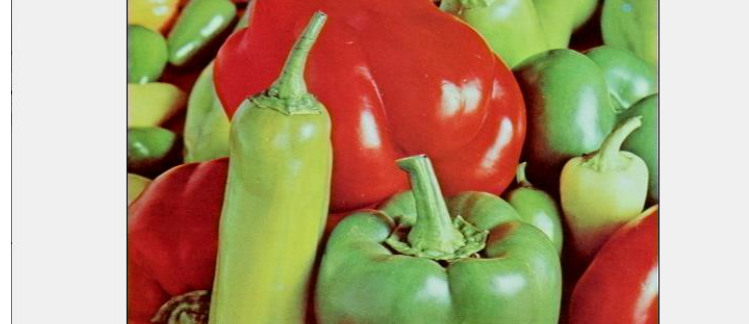
\includegraphics[width=81.90mm,height=89.10mm]{../../images/llm/page_072_img_01.png}%
\end{textblock*}

\end{document}
